\chapter{Kísérletek, eredmények} 
\label{ch:results}

Ebben a fejezetben értékelem ki és vetem össze különböző kísérleteim eredményeit.

\section{Mérőszámok}

A modellek teljesítményét F értékek alapján vetettem össze, egyrészt hangszerenként külön-külön, másrészt a hangszerenkénti átlagot véve is. Az F értékhez a következő metrikák vezettek el:

\begin{itemize}
\item \textbf{Pontosság (Accuraccy)} - a modell helyes előrejelzéseinek száma osztva az összes előrejelzés számával. Ez már magában egy jó mérőszám tud lenni, azonban multi-label osztályozások esetén érdemes a helytelen előrejelzések fajtájával is kalkulálni. Ezek a valótlan igazak (false positives) és valótlan hamisak (false negatives).
\begin{figure}[H]
  \centering
  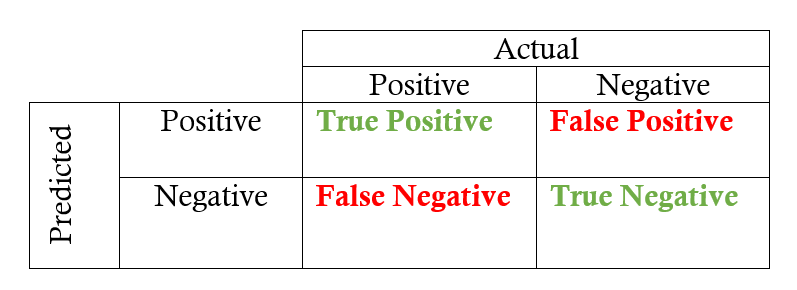
\includegraphics[width=\textwidth]{predictedactual.png}
  \caption{Előrejelzések fajtái, forrás: \cite{fscore}}
\end{figure}

\item \textbf{Veszteség (Loss)} - a veszteségfüggvény eredménye. A modell predikcióinak a valóságtól való eltérését összeadva kapjuk meg. A modell célja tanuláskor ennek az értéknek a minimalizálása.
\item \textbf{Precizitás (Precision)} - valós igaz predikációk száma osztva a valós és valótlan igazak számának összegével.
\item \textbf{Felidézés (Recall)} - valós igaz predikációk száma osztva a valós igaz és valótlan hamis predikációk összegével.
\begin{figure}[H]
  \centering
  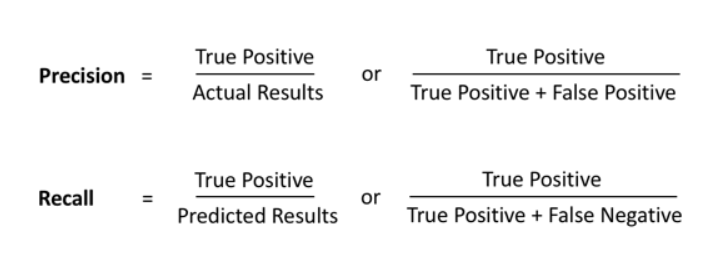
\includegraphics[width=\textwidth]{precisionrecall.png}
  \caption{Precizitás és felidézés, forrás: \cite{fscore}}
\end{figure}
\item \textbf{F érték (F score)} - a precizitás és felidézés értékek harmónikus közepe. Ez lesz tehát a meghatározó mérőszám modelljeink összevetésénél. \cite{fscore}

\begin{figure}[H]
  \centering
  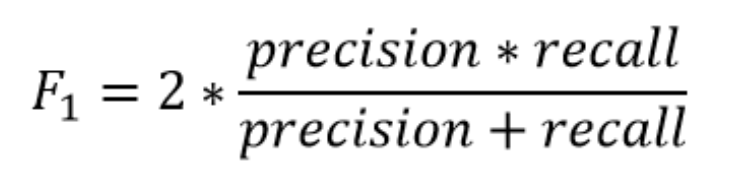
\includegraphics[width=6cm]{fscore.png}
  \caption{F score képlete, forrás: \cite{fscore}}
\end{figure}
\end{itemize}



\section{Eredmények}

A végső eredmények csak az OpenMIC datasettel kapcsolatos kísérleteket tartalmazzák. Az eredmények összevetésére a hangszerenkénti F score-okat használtam fel. Ez modellenként 19 hangszer, ami 19 különböző értéket jelent. Ezért minden modell végső összevetési alapjának két összesítő értéket választottam: az F-score-ok átlagát és a 0,70 feletti F score-t meghaladó hangszerek számát. Utóbbira a továbbiakban jól tanított hangszerként fogok hivatkozni. Saját intuícióm vezetett arra a következtetésre, hogy 0,70-es F score felett már életszerűen használható értékről beszélhetünk.

A továbbiakban a Modeling Baseline és a Shallow CNN architektúrák különböző eredményeit mutatom be.

\subsection{VGGish kiindulás}

Először a VGGish reprezentáció tekintetében tettem kísérleteket, mivel a Modeling Baseline eredeti implementációja ezt használta fel. Első lépésként ezt futtattam módosítás nélkül, majd lecseréltem a felhasznált RFC-t a saját CNN architektúrámra.

Az eredmények hangszerenként a \ref{fig:vggishbase} ábrán láthatóak. Az F-score-ok átlaga és a jól tanított hangszerek száma kicsivel magasabb volt a Modeling Baseline modellen, mint a Shallow CNN-en. Előbbi 0,79 átlag F score-t és 17 jól tanított hangszert, utóbbi 0,76 átlag F score-t és 14 jól tanított hangszert produkált.

\begin{figure}[H]
\centering
\begin{tikzpicture}
    \begin{axis}[
        width  = \textwidth,
        height = 8cm,
        major x tick style = transparent,
        ybar=0pt,
        bar width=4pt,
        ymajorgrids = true,
        ylabel = {F-score},
        symbolic x coords={Harmónika,Bendzsó,Basszusgitár,Cselló,Klarinét,Cintányér,Dob,Furulya,Gitár,Melodikus ütőhangszer,Mandolin,Orgona,Zongora,Szaxofon,Szintetizátor,Harsona,Trombita,Ukulele,Hegedű,Ének},
        xtick = data,
        x tick label style={rotate=90},
        scaled y ticks = false,
        legend cell align=left,legend style={
                at={(1,1.05)},
                anchor=south east,
                column sep=1ex}
    ]
        \addplot[style={bblue,fill=bblue,mark=none}]
            coordinates {(Harmónika, 0.68) (Bendzsó,0.72) (Basszusgitár,0.75)  (Cselló,0.79)  (Klarinét,0.52)  (Cintányér,0.93)  (Dob,0.75)  (Furulya,0.89)  (Gitár,0.97)  (Melodikus ütőhangszer,0.77)  (Mandolin,0.70)  (Orgona,0.60) (Zongora,0.93) (Szaxofon,0.83) (Szintetizátor,0.94) (Harsona,0.75) (Trombita,0.76) (Ukulele,0.72) (Hegedű,0.83) (Ének,0.93)};
        \addplot[style={rred,fill=rred,mark=none}]
            coordinates {(Harmónika, 0.76) (Bendzsó,0.74) (Basszusgitár,0.66) (Cselló,0.73) (Klarinét,0.52)  (Cintányér,0.88) (Dob,0.93) (Furulya,0.66) (Gitár,0.95)  (Melodikus ütőhangszer,0.79)  (Mandolin,0.64)  (Orgona,0.77) (Zongora,0.91) (Szaxofon,0.67) (Szintetizátor,0.89) (Harsona,0.77) (Trombita,0.71) (Ukulele,0.64) (Hegedű,0.76) (Ének,0.81)};
        \legend{Modeling Baseline VGGish ,Shallow CNN VGGish}
    \end{axis}
\end{tikzpicture}
\caption{Modeling Baseline és Shallow CNN kezdeti értékei optimalizációk nélkül VGGish reprezentáción} \label{fig:vggishbase}
\end{figure}


Ami még a \ref{fig:vggishbase} diagramról leolvasható, hogy a hangszerek között vannak jobban és kevésbé taníthatóak. Például a klarinét és mandolin mindkét modellen relatív alacsony F-értéket hozott. Ezzel szemben a gitár és zongora tanítása mindkét modell esetében 0.9 feletti F-értéket eredményezett.

A hangszereket vizsgálva a modellek között megjelentek nagyon hasonló és különböző értékek is. A legangyobb különbséget a Shallow CNN javára a dob mutatta, itt 0,75 állt szemben 0,93 értékkel, ami 0,18 F-score eltérés. A Modeling Baseline javára pedig a furulyával kapcsolatos számok jelentették a legnagyobb, 0,23 F-score eltérést. Itt 0,66 és 0,89 voltak az értékek.

\subsection{Optimalizáció}

Következő lépésként implementáltam a különböző előfeldolgozási adatoptimalizáló technikákat, mint például undersampling és normalizálió. Ezután szintén a VGGish reprezentáción futtatva a modellek teljesítménye javulást ért el: mindkét modell F score átlaga egyaránt 0,83-ra növekedett a korábbi 0,79-ről és 0,76-ról. Ezen felül a jól tanított hangszerek száma mindkét modell esetén elérte a maximális 20-at a korábbi 17 és 14 helyett. Ez a ShallowCNN számára magasabb relatív javulást jelent, ennek hangszerenkénti összevetése a \ref{fig:shallowcnnopt} ábrán látható.

\begin{figure}[H]
\centering
\begin{tikzpicture}
    \begin{axis}[
        width  = \textwidth,
        height = 10cm,
        major x tick style = transparent,
        ybar=0pt,
        bar width=4pt,
        ymajorgrids = true,
        ylabel = {F-score},
        symbolic x coords={Harmónika,Bendzsó,Basszusgitár,Cselló,Klarinét,Cintányér,Dob,Furulya,Gitár,Melodikus ütőhangszer,Mandolin,Orgona,Zongora,Szaxofon,Szintetizátor,Harsona,Trombita,Ukulele,Hegedű,Ének},
        xtick = data,
        x tick label style={rotate=90},
        scaled y ticks = false,
        legend cell align=left,legend style={
                at={(1,1.05)},
                anchor=south east,
                column sep=1ex}
    ] 
        \addplot[style={rred,fill=rred,mark=none}]
            coordinates {(Harmónika, 0.76) (Bendzsó,0.74) (Basszusgitár,0.66) (Cselló,0.73) (Klarinét,0.52)  (Cintányér,0.88) (Dob,0.93) (Furulya,0.66) (Gitár,0.95)  (Melodikus ütőhangszer,0.79)  (Mandolin,0.64)  (Orgona,0.77) (Zongora,0.91) (Szaxofon,0.67) (Szintetizátor,0.89) (Harsona,0.77) (Trombita,0.71) (Ukulele,0.64) (Hegedű,0.76) (Ének,0.81)};
       \addplot[style={ggreen,fill=ggreen,mark=none}]
            coordinates {(Harmónika, 0.74) (Bendzsó,0.81) (Basszusgitár,0.75) (Cselló,0.77) (Klarinét,0.72)  (Cintányér,0.93) (Dob,0.93) (Furulya,0.72) (Gitár,0.96)  (Melodikus ütőhangszer,0.79)  (Mandolin,0.79)  (Orgona,0.82) (Zongora,0.96) (Szaxofon,0.8) (Szintetizátor,0.96) (Harsona,0.81) (Trombita,0.81) (Ukulele,0.74) (Hegedű,0.84) (Ének,0.96)};
        \legend{Modeling Baseline VGGish ,Shallow CNN VGGish}
    \end{axis}
\end{tikzpicture}
\caption{Shallow CNN optimalizációk előtt és után VGGish reprezentáción} \label{fig:shallowcnnopt}
\end{figure}

\subsection{Alternatív reprezentációk}

//TODO MELSPEC, MFCC bevezetése, miért alacsonyabbak a számok, ml vs dl

\begin{figure}[H]
\centering
\begin{tikzpicture}
    \begin{axis}[
        width  = \textwidth,
        height = 10cm,
        major x tick style = transparent,
        ybar=0pt,
        bar width=4pt,
        ymajorgrids = true,
        ylabel = {macro f-score},
        symbolic x coords={Harmónika,Bendzsó,Basszusgitár,Cselló,Klarinét,Cintányér,Dob,Furulya,Gitár,Melodikus ütőhangszer,Mandolin,Orgona,Zongora,Szaxofon,Szintetizátor,Harsona,Trombita,Ukulele,Hegedű,Ének},
        xtick = data,
        x tick label style={rotate=90},
        scaled y ticks = false,
legend cell align=left,legend style={
                at={(1,1.05)},
                anchor=south east,
                column sep=1ex
        }
    ]
        \addplot[style={ppurple,fill=ppurple,mark=none}]
            coordinates {(Harmónika,0.45) (Bendzsó,0.39) (Basszusgitár,0.42) (Cselló,0.63)  (Klarinét,0.43)  (Cintányér,0.80)  (Dob,0.82)  (Furulya,0.41)  (Gitár,0.47)  (Melodikus ütőhangszer,0.52)  (Mandolin,0.39)  (Orgona,0.59) (Zongora,0.84) (Szaxofon,0.59) (Szintetizátor,0.51) (Harsona,0.47) (Trombita,0.59) (Ukulele,0.43) (Hegedű,0.57) (Ének,0.82) };

        \addplot[style={ggreen,fill=ggreen,mark=none}]
            coordinates {(Harmónika,0.46) (Bendzsó,0.46) (Basszusgitár,0.74) (Cselló,0.65)  (Klarinét,0.61)  (Cintányér,0.80)  (Dob,0.83)  (Furulya,0.54)  (Gitár,0.45)  (Melodikus ütőhangszer,0.57)  (Mandolin,0.57)  (Orgona,0.59) (Zongora,0.84) (Szaxofon,0.55) (Szintetizátor,0.73) (Harsona,0.54) (Trombita,0.44) (Ukulele,0.50) (Hegedű,0.68) (Ének,0.68) };
 	
        \legend{ML Mel,DL Mel}
    \end{axis}
\end{tikzpicture}
\caption{Modeling Baseline és Shallow CNN elődjének kezdeti értékei optimalizációk nélkül melspectogram reprezentáción} \label{fig:vggishbase}
\end{figure}